\documentclass{article}
\usepackage[utf8]{inputenc}

\usepackage{float}
\usepackage{caption}

\RequirePackage{tabularx}



\usepackage[table]{xcolor} 
\definecolor{myblue}{HTML}{CCF4FF}
\definecolor{myorange}{HTML}{FCAD68}

\usepackage{tikz}
\tikzstyle{decision} = [diamond, draw, fill=myblue, 
text width=4.5em, text badly centered, node distance=2.5cm, inner sep=0pt]
\tikzstyle{block} = [rectangle, draw, 
fill=myblue, align=center, rounded corners, minimum width = 2cm, minimum height=1cm]
\tikzstyle{line} = [draw, -latex']

\usepackage{todonotes}
\setuptodonotes{inline}
\usepackage{quotes}

\newcommand{\quotes}[1]{``#1''}

\input{../workflow/tikz_packages}

\begin{document}


\pagestyle{empty}
\large

\section*{\centering\hspace{-1cm}3D printers - Handleiding}
Na deze handleiding weet je hoe je efficient 3D print aanvragen kan verwerken. Er wordt vanuit gegaan dat je al weet hoe je een 3D printer werkt en dat je weet hoe je het filament vervangt, het bed schoonmaken, 3D bestanden sliced en de meest voorkomende errors weet aan te pakken.\\

Na deze handleiding weet je ook hoe je gestructureerd en efficient 3D print aanvragen kan verwerken. Het belangrijkste, als je wegloopt dan kan de volgende SA meteen weer door kunnen gaan waar jij was gebleven.

\section*{Termologie}
\noindent\textbf{Een print job}: Een folder met daarin alle bestanden gerelateerd aan het 3D print file (in 99\% van de gevallen een~.stl file) deze gerelateerde bestanden kunnen zijn: een mail gesprek, gcode, of een van de volgende files: \textit{afgekeurd.bat}, \textit{gesliced.bat}, \textit{printer\_aangezet.bat} of \textit{printer\_klaar.bat}.

\section*{Globaal Overzicht}
\begin{center}
\scalebox{0.7}{
  \hspace{0.5cm}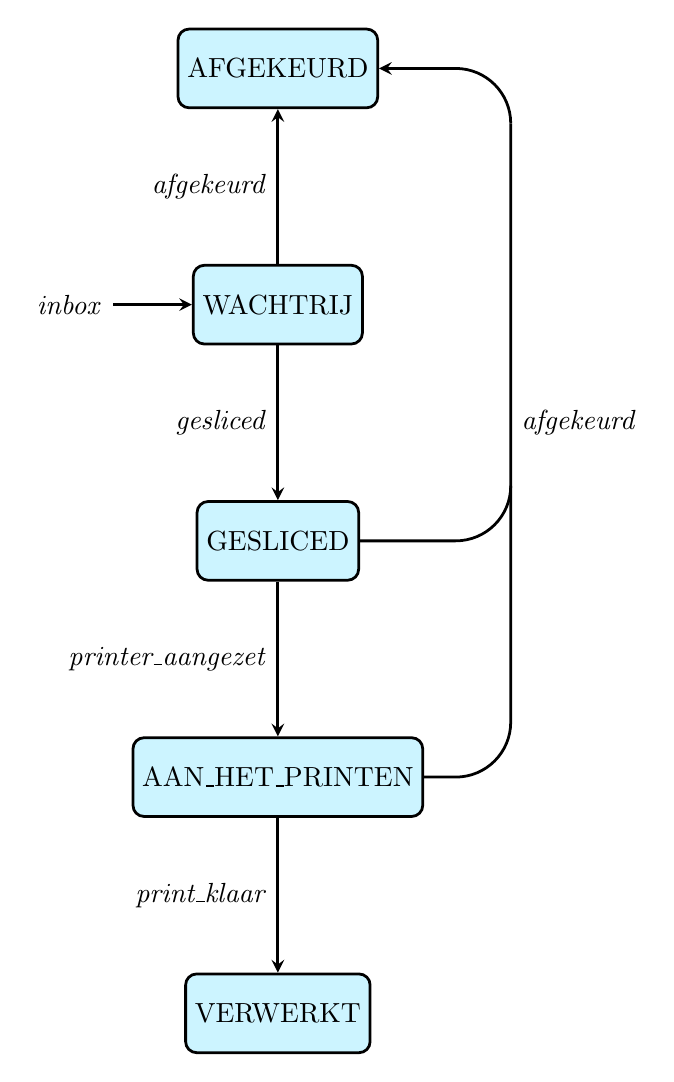
\begin{tikzpicture}[node distance = 3.0cm, line width=1pt]
    % Nodes
    \node [block] (wachtrij) {WACHTRIJ};
    \node [block, above of=wachtrij]  (afgekeurd) {AFGEKEURD};
    \node [block, below of=wachtrij]  (gesliced) {GESLICED};
    \node [block, below of=gesliced]  (aan_het_printen) {AAN\_HET\_PRINTEN};
    \node [block, below of=aan_het_printen] (verwerkt) {VERWERKT};

    % define lengths
    \pgfmathsetlengthmacro{\alpha}{0.7cm} % curve radius
    \pgfmathsetlengthmacro{\negalpha}{-\alpha}
    \pgfmathsetlengthmacro{\beta}{0.4cm} % straight bit before the curve

    % arrows
    \draw[>=stealth, ->, line width=1.0pt] ([xshift=-1.0cm]wachtrij.west) to node[xshift=-0.5cm,left]{\textit{inbox}} (wachtrij.west);
    \draw[>=stealth, ->, line width=1.0pt] (wachtrij.north) to node[left] {\textit{afgekeurd}} (afgekeurd.south);
    \draw[>=stealth, ->, line width=1.0pt] (wachtrij.south) to node[left] {\textit{gesliced}} (gesliced.north);
    \draw[>=stealth, -, line width=1.0pt] (aan_het_printen.east) -- ++(\beta,0)  to[out=0, in=-90] ++(\alpha, \alpha) -- node[right]{\textit{afgekeurd}} ([xshift=\alpha+\beta,yshift=\negalpha]afgekeurd.east -| aan_het_printen.east);
    \draw[>=stealth, <-, line width=1.0pt] (afgekeurd.east) -- ([xshift=\beta] afgekeurd -| aan_het_printen.east)  to[out=0, in=90] ++(\alpha,\negalpha);
    \draw[>=stealth, -, line width=1.0pt] (gesliced.east) -- ([xshift=\beta] gesliced -| aan_het_printen.east) to[out=0, in=-90] ++(\alpha,\alpha);
    \draw[>=stealth, ->, line width=1.0pt] (gesliced.south) to node[left] {\textit{printer\_aangezet}} (aan_het_printen.north);
    \draw[>=stealth, ->, line width=1.0pt] (aan_het_printen.south) to node[left] {\textit{print\_klaar}} (verwerkt.north);

  \end{tikzpicture}

}
\end{center}
Een print job wordt aangemaakt door op de snelkoppeling \textit{inbox} (op het bureaublad) te klikken. Dit maakt een print job aan in de WACHTRIJ folder, als alles goed gaat verplaatst een print job zich via WACHTRIJ $\rightarrow$ GESLICED $\rightarrow$ AAN\_HET\_PRINTEN $\rightarrow$ VERWERKT. Mocht er ergens wat mis gaan dan gaat de print job naar de AFGEKEURD folder. Deze folders zijn subfolders van de 3D PRINT HOME folder op het bureaublad.

\section*{Binnengekomen mails omzetten tot print jobs}
(nogmaals) een print job wordt aangemaakt door op de snelkoppeling \textit{inbox} (op het bureaublad) te klikken. Als er nieuwe mails in de inbox folder van 3d-iws@tudelft.nl zijn binnengekomen, dan worden nieuwe print jobs aangemaakt in de folder WACHTRIJ (subfolder van 3D PRINT HOME op het bureaublad). In Outlook zullen deze mails van Inbox naar Verwerkt worden verplaatst.\\

LET OP: wordt er binnen de CMD aangegeven \quotes{Press any key to continue...} of \quotes{Press enter to continue...} Druk dan ook op \quotes{any key} or \quotes{enter} en KLIK NIET op het rode kruis bovenin. Er gebeurd namelijk nog vanalles nadat je op \quotes{any key} of \quotes{enter} hebt gedruk, dit gebeurd niet als je op het rode kruis klikt.\\

\section*{Slicen}
De print jobs in de wachtrij zullen gesliced moeten worden. Slice de 3D print bestanden met de prusa slicer, klik daarna op het gesliced.bat file in de print job, deze verplaats de print job van WACHTRIJ naar de GESLICED folder. 

\section*{Afkeuren}
Lukt het slicen niet of kan de 3d print aanvraag om andere reden niet worden gemaakt, keur de print job af door op de afgekeurd.bat functie te klikken. Deze functie vraagt waarom een 3D print bestand niet kan worden geprint. Vul een reden in en druk op enter, een reactie mail komt tevoorschijn (het kan zijn dat deze achter andere programma's tevoorschijnt komt). Verzend de mail, als je geen mail wil verzenden, klik bij de mail popup op het rode kruisje rechtsboven. Hierna zal de print job naar de AFGEKEURD folder verplaatst worden.

\section*{Zet Printer Aan}
Zet een printer aan door de gcode te slepen naar een printer in de webbrowser. Klik hierna op printer\_aangezet.bat, de print job word naar de AAN\_HET\_PRINTEN folder verplaatst.\\

Zitten er meerdere g-code bestanden in de print job, dan krijg je de vraag welke gcode bestanden nog geprint moeten worden in de toekomst. De print job zit dan voor een gedeelte in de AAN\_HET\_PRINTEN en de GESLICED folders. 

\section*{Print Klaar}
Als een print klaar is, klik op de print\_klaar.bat functie. Een mail popup verschijnt, verzend de mail. De print job wordt naar de VERWERKT folder verplaatst. 


\section*{Let Hier Op!}
\begin{itemize}
  \item Vraagd de CMD press any key to continue... of press enter to continue... Klik dan niet de CMD weg, druk op \quotes{any key} of \quotes{enter}. Er gebeurd nog wel iets nadat je op enter/any key druk. Dit gebeurd niet als je op kruisje klikt
  \item Klikken op zet\_printer\_aan.bat doet niet zoveel (verplaatst de print job van GESLICED naar AAN\_HET\_PRINTEN) toch is het belangrijk voor de boekhouding, de volgende SA weet niet of dit nou wel of niet al aan het printen was
  \item Check de mail die mensen sturen, hier staat vaak info in die belangrijk is voor je om te weten, zoals hoe vaak een onderdeel geprint moet worden.
\end{itemize}

\section*{Print jobs vanuit een lokaal bestand}
Het is mogelijk via een usb stick een 3D print bestand aan te leveren. Dit kan met de selecteer\_bestand snelkoppeling op het bureaublad. Omdat dit niet de gewenste manier is (dat is via de mail) is dit beschermd met een wachtwoord. Deze methode is bedoeld voor grote groepen zoals alle project groepen van WB1. 

\section*{IO-bit unlocker}
Bij het verplaatsen van een print job wordt eerst de print job naar een nieuwe locatie gekopieerd, daarna wordt de oude map verwijdert. Het verwijderen van deze map gebeurd met het programma IO-bit unlocker wat een bestand kan verwijderen ook al is het geopend in de prusa slices, of een mail staat open. Dit vind windows 10 niet altijd leuk, het kan dus zijn dat windows crashed en opnieuw opstart. Geen probleem, IO-bit unlocker en windows zijn geen vrienden.

\section*{Job Tracker}
De job tracker houd bij in welke folder een print job hoort te staan. Mocht er iets fout gaan op een of andere manier, dan repareerd de job tracker het systeem. Bijvoorbeeld een print job staat in de WACHTRIJ maar ook in de GESLICED folder, dan zal de job tracker verwijdert een van deze 2 jobs verwijderen. Ook verwijdert de job tracker jobs uit de AFGEKEURD en VERWERKT folder die ouder zijn dan 2 weken.\\  

Dat was hem, succes!


\end{document}


